\documentclass[]{article}

% math packages
\usepackage{amsmath}
\usepackage{amsthm}
\usepackage{bm}

% for coloring in a table
%\usepackage[table,xcdraw]{xcolor}

% including graphics
\usepackage{graphicx}
\graphicspath{ {./images/} }

% drawing graphs
\usepackage{tikz-cd}
\usepackage{tikz}
\usetikzlibrary{shapes.geometric, arrows}
\tikzstyle{startstop} = [rectangle, rounded corners, minimum width=3cm, minimum height=1cm,text centered, draw=black, fill=red!10]
\tikzstyle{arrow} = [thick,->,>=stealth]

% hyperlinks
\usepackage{hyperref}

% some useful shortcuts
\DeclareMathOperator*{\argmax}{argmax}
\newcommand{\indep}{\perp\!\!\!\!\perp}
\newcommand{\blambda}{{\bm{\lambda}}}
\newcommand{\btheta}{{\bm{\theta}}}
\newcommand{\bpsi}{{\bm{\psi}}}

\newcommand{\by}{\mathbf{y}}

\usepackage{setspace}
\doublespacing

\usepackage{natbib}
\bibliographystyle{rusnat}

% Editing macros
\usepackage{color}
\newcommand\cmnt[2]{\qquad{{\color{red} \em #1---#2} \qquad}}
\newcommand\cmntM[1]{\cmnt{#1}{Miratrix}}
\newcommand\cmntC[1]{\cmnt{#1}{Che}}
\newcommand\awk{{{\color{red} {$\leftarrow$ Awkward phrasing}}\qquad}}
\newcommand\cmntMp[1]{{\color{red} $\leftarrow$ {\em #1 -Miratrix} \qquad}}



%opening
\title{On power analyses for individual site impacts in multisite trials}
\author{Jonathan Che \& Luke Miratrix}

\begin{document}

\maketitle


\section{Background}

Power analyses for multisite trials generally ensure that a given design will achieve desired levels of power for the overall average treatment effect $\tau$ across all sites. [TODO: add references for prior power analysis stuff for multisite trials, like Kristen’s power formula work, formulas for detecting cross-site impact heterogeneity, etc?] 

In many applications, however, site stakeholders may be interested in estimating treatment effects $\tau_j$ at the individual sites $j$ as well, for sites $j = 1, \dots, J$.
Analysts typically use multilevel models (MLMs) to produce partially pooled estimates of $\tau_j$.
For each site, these models ``borrow strength'' from the other sites, resulting in estimates $\hat{\tau}_j$ that are shrunken toward the estimated overall average treatment effect $\hat{\tau}$.
Standard Bayesian procedures may be used to construct credible intervals to conduct inference on the individual site-level effects.

The interpretation of these credible intervals requires some nuance.
There is an extensive literature concerning the construction of such intervals for individual site effects under shrinkage \citep{casella2012shrinkage}.
These intervals typically possess a so-called Empirical Bayes coverage property \citep{morris1983parametric}, i.e., they guarantee coverage for the collection of $\tau_j$ values \textit{on average} across all $J$ sites, not coverage for each individual $\tau_j$.
These guarantees may not be sufficient for stakeholders in multisite trials interested in understanding the effect of an experimental treatment at their particular site.
Overall, the question of inference for individual $\tau_j$ values in multilevel models remains fairly open \citep{armstrong2020robust}, with limited guidance about best practices.

\section{Objective}

In this paper, we first clarify how to interpret the individual site-level effect estimates produced by MLMs.
We then conduct power analyses to explore how well MLMs can detect hypothesized effects for individual sites in multisite trials.
Similar power analyses have previously been conducted for the overall average treatment effect and cross-site variation in multisite trials \citep{raudenbush2000statistical}, but not for individual site-effect estimates, to the best of our knowledge.

% Two ideas to add:
% Idea 1: we're assuming exchangeability, so before the trial is run, everyone is the same to some extent?
% Idea 2: post-hoc power analyses are bad \href{https://statmodeling.stat.columbia.edu/2018/09/24/dont-calculate-post-hoc-power-using-observed-estimate-effect-size/}{says Gelman}

% We're doing a weird mix of pre- and post-trial stuff.
% In terms of coverage, things make sense.
% One idea: before we've run the analysis, what's the coverage of my intervals for sites with a true effect size of $\tau_j = 0.3$?
% Another idea: before we've run the analysis, what's the coverage of my intervals for sites with estimated $\hat{\tau}_j = 0.3$?

% In terms of power, things get weird.
% One idea: before we've run the analysis, what's the power of my procedure to detect effects at sites with $\tau_j = 0.3$?
% Another idea: before we've run the analysis, what's the power of my procedure to detect effects at sites with $\hat{\tau}_j = 0.3$?

% Is this second idea useful?
% Say I've run the trial and my observed $\hat{\tau}_j = 0.3$.
% The power analysis isn't useful at this point; I just have whatever interval I have, which says what it says.

% Something to note: power conditional on tau-hat depends strongly on the distribution of the $\tau_j$ values.
% Power conditional on $\tau_j$ depends less strongly on that, perhaps?

% The issue with post-hoc power analyses is...
% Plugging in $\hat{\tau}$ for $\tau$ is bad.
% Here, we're treating $\hat{\tau}_j$ and $\tau_j$ as completely different things, so it avoids those issues.


% Arc of the story: MLMs are bad if we're considering power at individual $\tau_j$ values.
% This is because individual CIs are by definition biased for individual $\tau_j$ values.
% This bias leads to weird coverage properties, and bad inferences.

% MLMs are good if we're considering power at individual $\hat{\tau}_j$ values.
% This is because shrinkage helps; based on the collection of sites, we can get information that an extreme $\hat{\tau}_j$ value is likely due to measurement error/noise, and not an extreme signal $\tau_j$.
% By pooling information, we are more likely to reject the null for any particular $\hat{\tau}_j$.

% TODO: study interval length

\section{Research Design}

We conduct a simulation study to explore power for individual site-level effects. 
We repeatedly simulate data under a normal hierarchical model where we vary four data-generating parameters: the average size of each site $\bar{n}$, the number of sites $J$, the true overall average treatment effect $\tau$, and the true cross-site variation in site-level effects $\sigma^2_\tau$.
For each simulated dataset, we run four models: a normal Bayesian hierarchical model; a fixed-intercept, random-coefficients (FIRC) model \citep{bloom2017using}; a random-intercepts, random-coefficients (RIRC) model; and a separate t-test for each site. Finally, we record each model’s estimates of site-level effects and their associated credible intervals.

\section{Findings/Results}

In a standard power analysis, the analyst posits an effect size $c$ and computes power (at level $\alpha$), possibly for a range of sample sizes.
An analogous procedure for site-level effects in a multisite trial would be to fix a true site-level effect $c$ and compute power as the probability of rejecting the null when the true site-level effect is $c$.
Figure \ref{fig:power_plot} visualizes the results of a power simulation under this setup.
The power of a one-sided hypothesis test for a positive effect ($\alpha = 0.1$) is plotted against the true site-level effect size $\tau_j$.
% We fix $J = 100$ and $\tau = 0.2$, and vary $\bar{n}$ and $\sigma_\tau$ along the facets.
The dashed reference lines are at $0.1$ and $0.8$; 
ideally, the power curves would all be less than $\alpha = 0.1$ for $\tau_j \leq 0$ to ensure test validity and as high as possible for $\tau_j > 0$ to maximize test power.
\begin{figure}[ht]
	\centering
	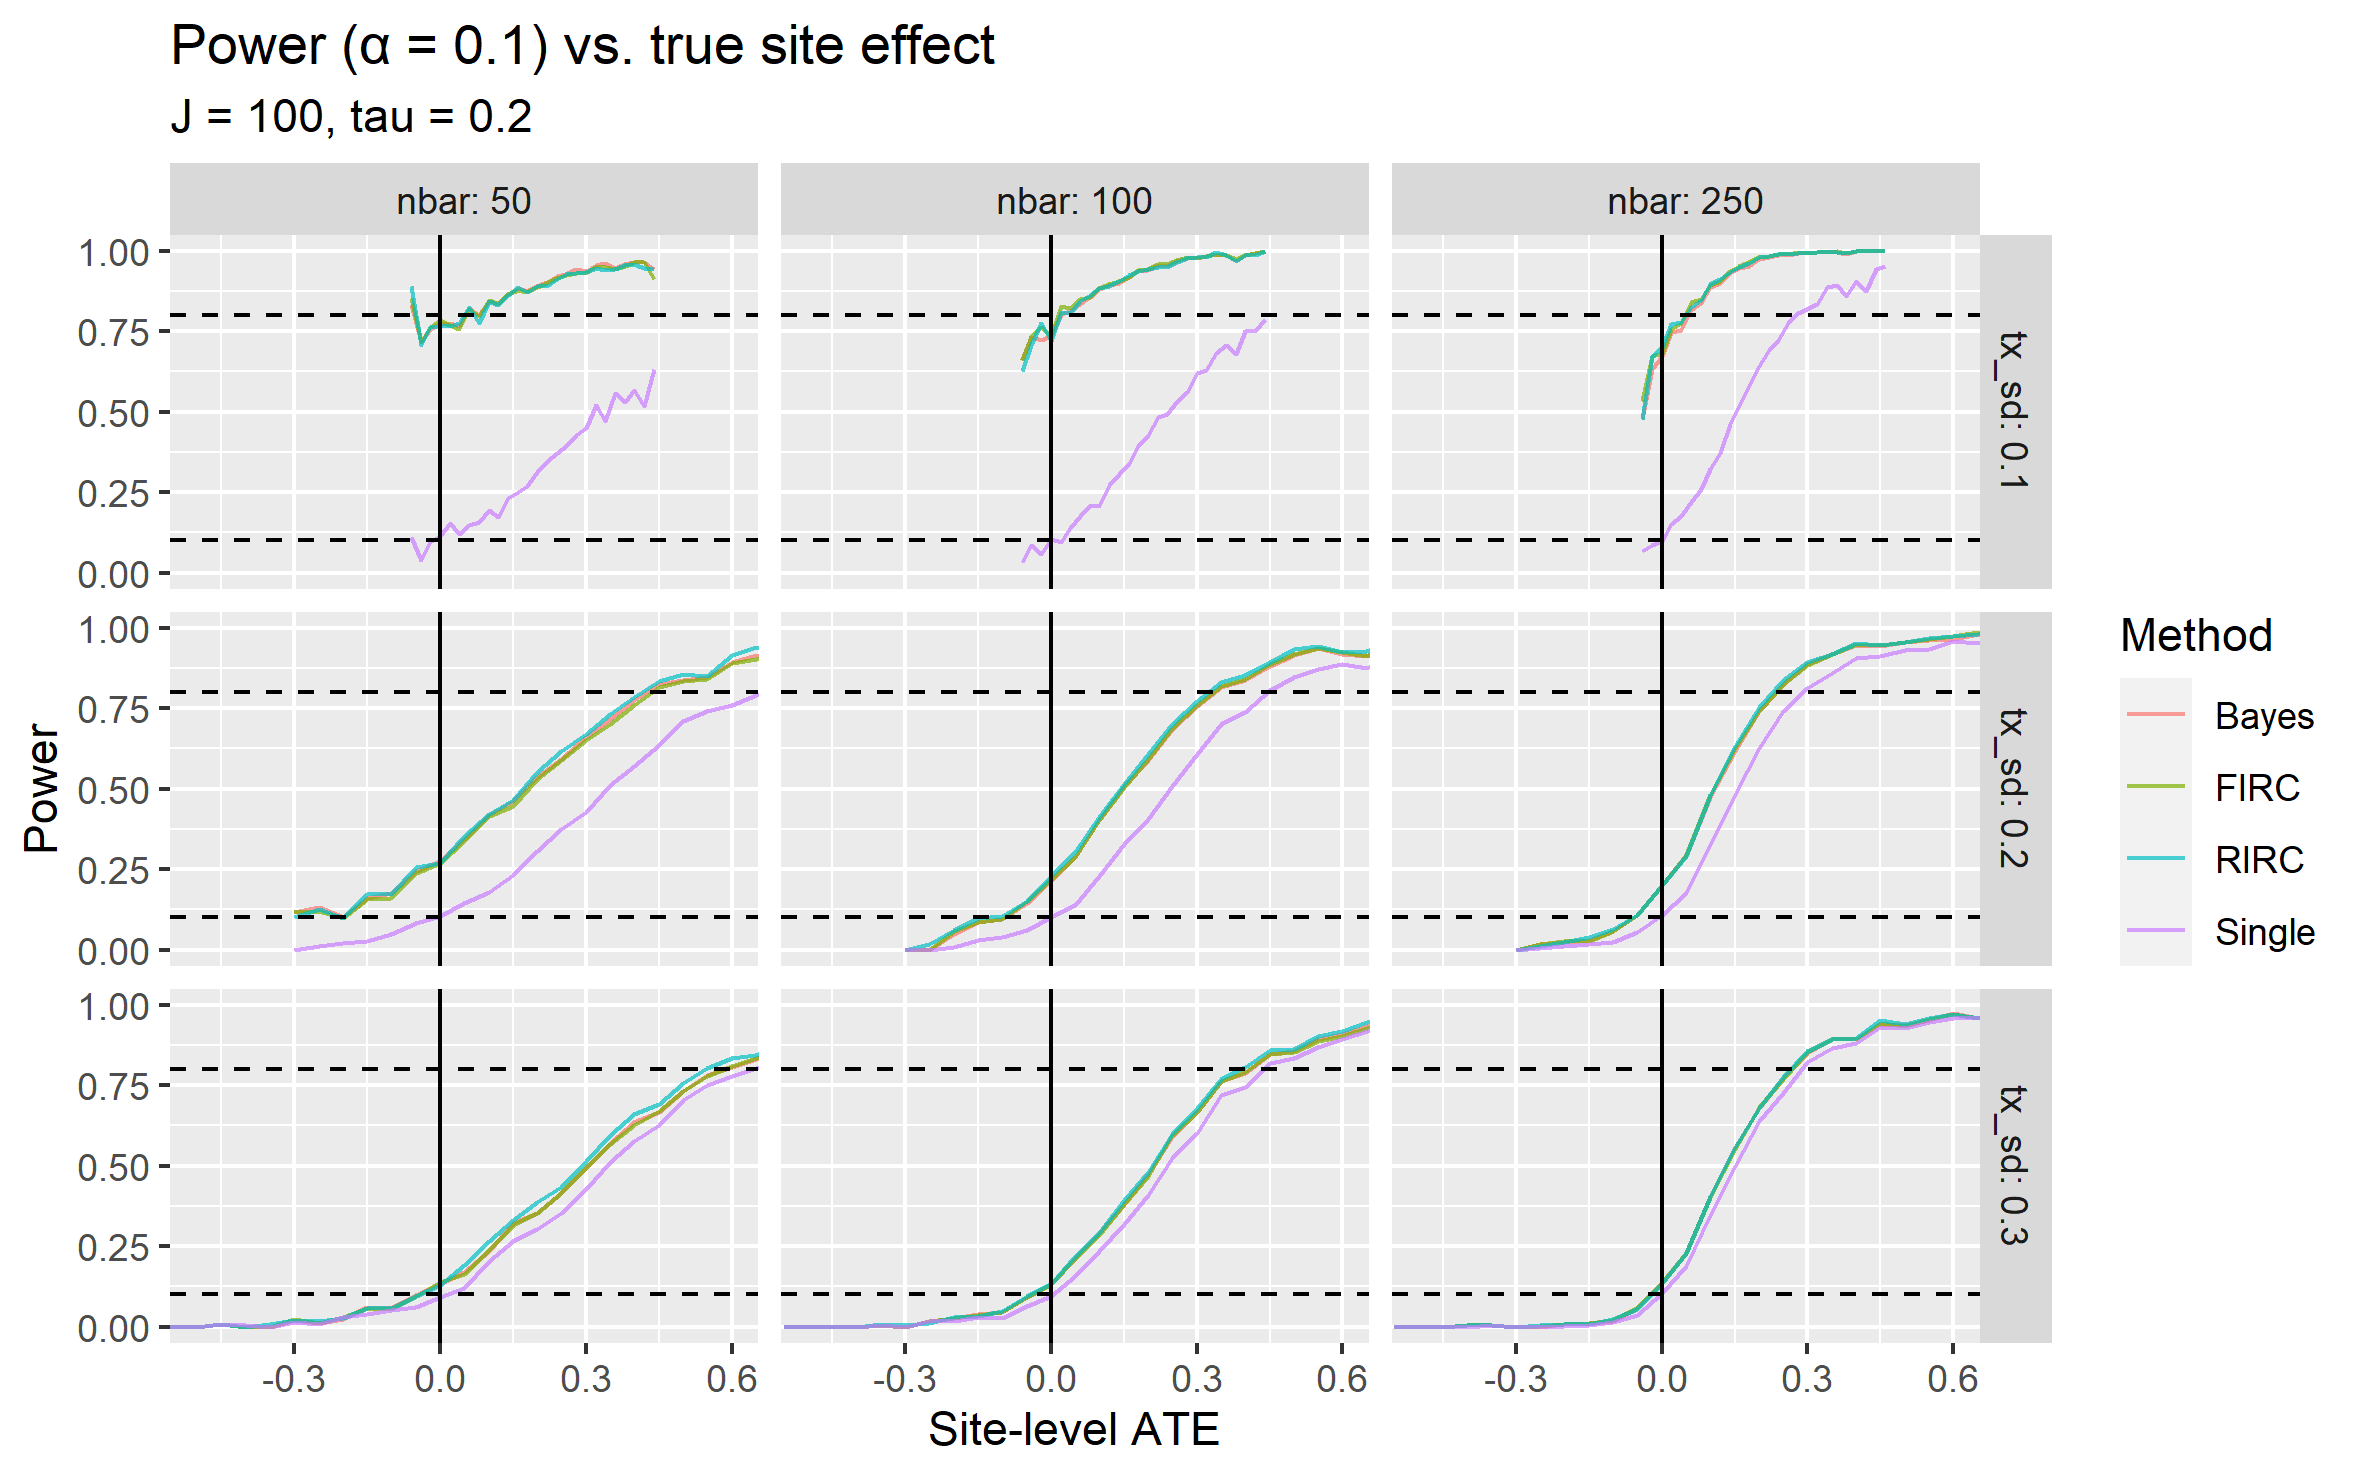
\includegraphics[width=\textwidth]{power_plot_J100}
	\caption{Plot of power (at $\alpha = 0.1$) vs. true site ATE}
	\label{fig:power_plot}
\end{figure}

We see that while using MLMs improve power relative to estimating each site separately, these improvements often come at the cost of test validity.
This result holds for all of the MLMs, and is particularly extreme when $\sigma_\tau = 0.1$, where the false positive rate for sites with negative $\tau_j$ values is nearly 80\%.

This behavior is expected for MLMs when power is computed at fixed values of $\tau_j$.
In this example, the MLMs naturally shrink estimates for sites with unusually small $\tau_j$ values toward the estimated overall mean, which is closer to $\tau = 0.2$.
The MLMs therefore estimate more positive effects for sites with negative $\tau_j$ values, resulting in many false rejections, particularly when shrinkage is strong.
Generally speaking, we implement MLMs in order to systematically shrink point estimates toward the overall mean.
This naturally results in interval undercoverage (and falsely inflated power) for sites with true $\tau_j$ values far from the overall mean.

In other words, MLMs have poor Frequentist coverage properties for fixed $\tau_j$ values.
MLMs, however, have excellent coverage properties and power \textit{for fixed $\hat{\tau}_j$ values} when they are well-specified.
Figure \ref{fig:power_plot_cond} is the same as Figure \ref{fig:power_plot}, except now power is computed for fixed $\hat{\tau}_j$ values rather than for fixed $\tau_j$ values.
\begin{figure}[ht]
	\centering
	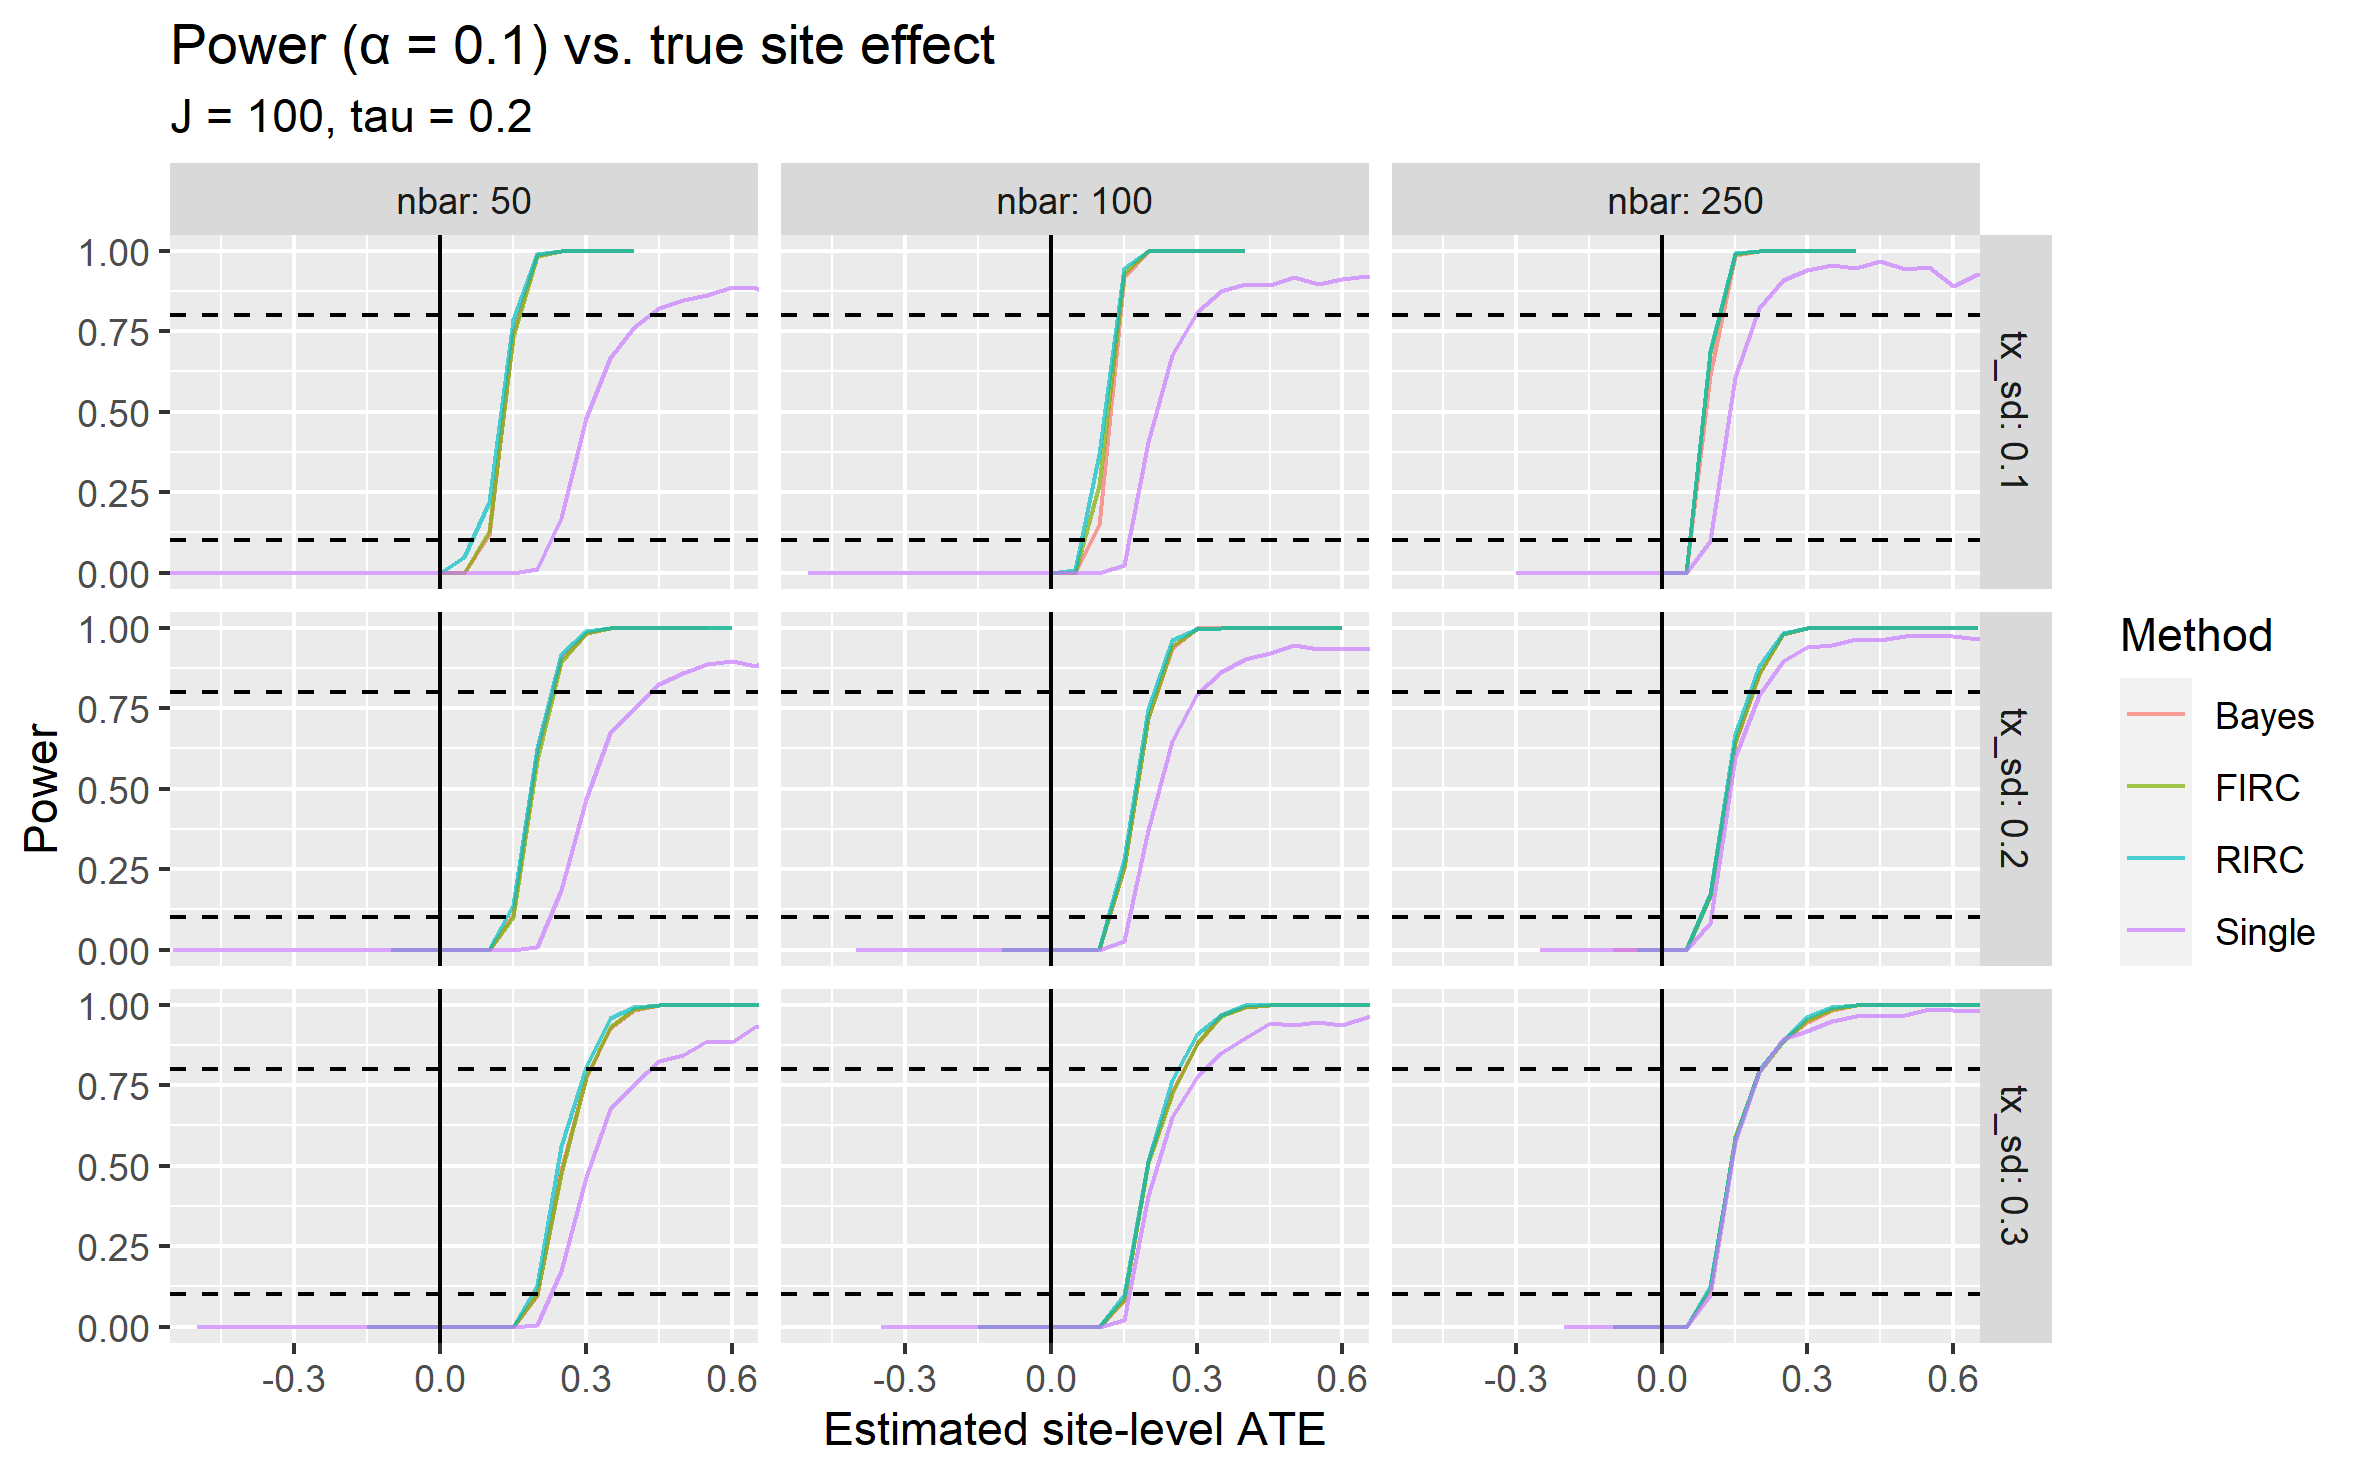
\includegraphics[width=\textwidth]{cond_power_1sided}
	\caption{Plot of power (at $\alpha = 0.1$) vs. estimated site ATE}
	\label{fig:power_plot_cond}
\end{figure}



If MLM intervals are biased for $\tau_j$ values, why are they good to use?
We can define another analogue of power: probability of rejecting null given $\hat{\tau}_j$.
Figures 3 and 4 show how this works out.
For each fixed $\hat{\tau}_j$ value, MLM coverage grows to become good, and MLMs have much better power.
Note that this is not post-hoc power; we're treating tau-hat as a completely separate thing from tau.

The idea is shown in Figure 5.
This is the whole idea behind MLMs; shrinkage is by definition bias, but it produces better overall estimates in terms of RMSE (not shown here).
If we're interested in individual sites, better RMSE doesn't necessarily guarantee us anything for each individual site (plus it doesn't care about inference).
We only have average coverage guarantees.

At each tau-j value, tau-hat is biased due to shrinkage.
At each tau-hat value, single-site estimates are biased because they don't appropriately account for the fact that in the population, extreme tau-j values are unlikely.
MLMs shrink to account for this, so at each tau-hat value, the average tau-j is the same as tau-hat.

\section{Conclusions}

In many multisite trials, practitioners may be interested in using the estimates produced by MLMs to conduct inference on treatment effects at individual sites.
While MLMs can improve estimation of the overall average treatment effect and cross-site effect heterogeneity, they do not generally improve inferences for individual sites.
In particular, shrinkage can lead to undesirable Frequentist validity and coverage properties, particularly in settings where shrinkage is high.
Practitioners interested in improving power to detect effects at individual sites should aim to make the individual site's estimate more precise, rather than aiming to add other sites to the analysis.

\bibliography{refs.bib}
	
\end{document}